\documentclass[conference]{IEEEtran}

\IEEEoverridecommandlockouts

% Turkce karakterler icin.
\usepackage[utf8]{inputenc}
\usepackage[T1]{fontenc}
\usepackage{cite}
\usepackage{amsmath,amssymb,amsfonts}
\usepackage{algorithmic}
\usepackage{graphicx}
\usepackage{textcomp}
\usepackage{xcolor}
\usepackage{booktabs}
\usepackage{url}
\usepackage{array}

% correct bad hyphenation here
\hyphenation{op-tical net-works semi-conduc-tor}

\begin{document}

\IEEEpubid{\makebox[\columnwidth]{979-8-3503-8896-1/24/\$31.00~\copyright~2024 IEEE\hfill} 
    \hspace{\columnsep}\makebox[\columnwidth]{}}

\title{Destek Vektör Regresyonu ile Yüksek Verimli Hapsedilme Kaybı Tahmini\\
    High-Efficiency Confinement Loss Prediction via Support Vector Regression}

\author{\IEEEauthorblockN{Anonymous Authors}
}

\maketitle

\begin{ozet}
Fotonik Kristal Fiber (PCF) tabanlı Yüzey Plazmon Rezonans (SPR) sensör tasarımı, hesaplama maliyeti yüksek simülasyonlara dayanır. Literatürde veri artırma için Üretken Çekişmeli Ağların (GAN) kullanımı önerilse de, sentetik verilerin fiziksel olmayan gürültü üreterek model performansını düşürdüğü bir Artırma Paradoksu saptadık. Bu çalışmada, sentetik veriye ihtiyaç duymadan 0,121 Ortalama Kare Hata ile GAN artırılmış sinir ağlarını 0,314 hataya kıyasla yüzde 60 oranından fazla geride bırakan Bayesyen optimize edilmiş bir Destek Vektör Regresyonu (SVR) modeli öneriyoruz. SHAP (SHapley Additive exPlanations) analizi ile dış kaplama geometrisinin hapsedilme kaybını yönlendiren birincil faktör olduğunu belirledik. Ayrıca Monte Carlo analizi, sensörün pitch parametresinin spektral kararlılık için en kritik unsur olduğunu ve yüzde 3 üretim toleransında 1,23 nm rezonans titremesine yol açtığını göstermektedir.
\end{ozet}

\begin{IEEEanahtar}
Fotonik kristal fiber; yüzey plazmon rezonans; destek vektör regresyonu; açıklanabilir yapay zeka; Bayesyen optimizasyon.
\end{IEEEanahtar}

\begin{abstract}
The design of Photonic Crystal Fiber based Surface Plasmon Resonance sensors relies on computationally expensive simulations. While recent studies propose Generative Adversarial Networks (GAN) for data augmentation, we demonstrate an Augmentation Paradox where GAN generated samples introduce non physical noise that degrades rigorous kernel models. Instead, we propose a lightweight Bayesian optimized Support Vector Regression model. Achieving a Mean Squared Error of 0.121, our Support Vector Regression outperforms GAN augmented neural networks by over 60 percent without requiring synthetic data. Utilizing SHapley Additive exPlanations (SHAP) values, we identify the outer cladding geometry as the primary driver of confinement loss. Furthermore, Monte Carlo robustness analysis reveals the sensor pitch is most critical for spectral stability, causing a 1.23 nm resonance jitter at a 3 percent manufacturing tolerance. 
\end{abstract}

\begin{IEEEkeywords}
Photonic crystal fiber; surface plasmon resonance; support vector regression; explainable AI; Bayesian optimization.
\end{IEEEkeywords}

\IEEEpeerreviewmaketitle

\IEEEpubidadjcol

\section{Introduction}
Photonic Crystal Fibers (PCFs) coated with plasmonic materials form highly sensitive Surface Plasmon Resonance (SPR) sensors for chemical and biological detection. Traditionally, optimizing these sensors involves the full vectorial finite element method (FV-FEM) to solve Maxwell's equations. While precise, FV-FEM is computationally prohibitive, making iterative geometric optimization extremely slow.

Machine Learning (ML) has emerged as a surrogate modeling alternative to address this bottleneck. Chugh et al. \cite{b2} pioneered the use of Artificial Neural Networks (ANNs) to accelerate PCF computations, but such deep learning models require large training datasets. Zelaci et al. \cite{b1} addressed this by using a Wasserstein Generative Adversarial Network with Gradient Penalty (WGAN-GP) to synthesize training samples, achieving a Mean Squared Error (MSE) of 0.314. Additionally, interpretability techniques like SHapley Additive exPlanations (SHAP) have been applied to identify critical parameters like gold thickness \cite{b3}, alongside traditional models like k-nearest neighbor regression for bent fibers \cite{b4}.

We hypothesize that PCF-SPR confinement loss, characterized by sharp non-linear resonances and inherently small datasets ($N < 500$), is better suited for boundary-focused algorithms rather than deep learning. We evaluate Bayesian-optimized Support Vector Regression (SVR) and Gaussian Process Regression (GPR) against the GAN-ANN baseline. SVR builds regression margins based exclusively on extreme boundary cases, while GPR maps mathematical covariance without overfitting. We demonstrate that these lightweight models significantly outperform augmented Deep Neural Network (DNN) benchmarks without requiring synthetic data. Furthermore, we empirically prove an ``Augmentation Paradox'': microscopic numerical noise in GAN-generated data warps the SVR hyperplane and degrades GPR covariance matrices, actively harming predictive performance.

Finally, to ensure practical utility, we apply SHAP analysis to deconstruct regression outputs and isolate the marginal contributions of each physical feature, revealing how specific parameters drive evanescent field leakage. 

The remainder of this paper is organized as follows: Section II describes the numerical modeling and dataset generation. Section III presents the methodology. Section IV discusses predictive performance, benchmarks, and manufacturing robustness. Section V provides engineering validation using SHAP, and Section VI concludes the paper.

\section{Numerical Modeling and Dataset Generation}

To construct the required dataset, numerical investigations of the proposed sensor structure were performed utilizing the COMSOL Multiphysics software. Utilizing Perfectly Matched Layers (PMLs), the Full Vectorial Finite Element Method (FV-FEM) was the primary numerical solver for these simulations. Illustrated in Fig. \ref{Fig:cross_section} is the cross-section of the proposed structure; the sensor comprises an analyte channel acting as the sensing medium, a plasmonic Gold (Au) layer, and cladding air holes of various dimensions. Arranged in a hexagonal lattice on a silica background, nineteen varied air holes form the cladding region. The radius of each hole was defined as $r_1= 0.225\,\mu\text{m}$, $r_2= 0.375\,\mu\text{m}$, $r_3 = 0.175\,\mu\text{m}$, and $r_c = 0.075\,\mu\text{m}$, while the pitch ($\Lambda$) remained fixed at $2\,\mu\text{m}$.

\begin{figure}[htbp]
	\centering
	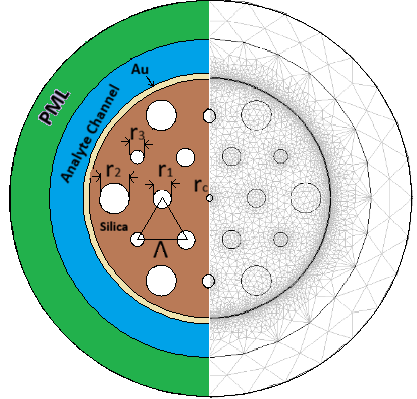
\includegraphics[width=.7\linewidth]{Figx}
	\caption{The cross-section of the proposed PCF based SPR sensor.}
	\label{Fig:cross_section}
\end{figure}

Light is effectively confined within the core region during the fundamental mode propagation. However, a specific fraction of light must leak toward the plasmonic layer to satisfy the conditions for resonance phase-matching, where the sensitivity measurement occurs. In this context, the light guidance is controlled by the various sized cladding holes, where each set of holes influences the sensor’s propagation characteristics. The Gold (Au) material, serving as the plasmonic layer, was set to a thickness of $40\,\text{nm}$, with permittivity values sourced from the Johnson and Christy data \cite{b6}. To determine the refractive index of the silica material, the Sellmeier Equation was applied \cite{b5}:

\begin{equation}
	n^2(\lambda) = 1 + \frac{B_1\lambda^2}{\lambda^2 - C_1} + \frac{B_2\lambda^2}{\lambda^2 - C_2} + \frac{B_3\lambda^2}{\lambda^2 - C_3}
	\label{eq:sellmeier}
\end{equation}

where $\lambda$ represents the operating wavelength, $n$ is the Refractive Index (RI), and $B_{1,2,3}$ and $C_{1,2,3}$ are the standard Sellmeier constants. Confinement losses reach their peak during the resonance phase-matching condition. Consequently, the precise calculation of these losses is vital, for which the following equation was utilized in this study \cite{b1}:

\begin{equation}
	L_c = \frac{40\pi}{\ln(10)\lambda} \text{Im}(n_{eff}) \times 10^4 \, [\text{dB/cm}]
	\label{eq:confinement_loss}
\end{equation}

where $\text{Im}(n_{eff})$ denotes the imaginary part of the effective RI. 

\section{Methodology}
In this section, we detail the data preparation pipeline and the mathematical foundations of the regression models employed in this study. In this study, the same dataset used in \cite{b1} is employed. Given the high-fidelity nature of the FV-FEM simulations, the methodology focuses on maintaining physical consistency while maximizing predictive accuracy in a small-data regime.

\subsection{Dataset and Preprocessing}
The FV-FEM numerical analysis provided a labeled dataset containing 432 samples. The input feature space comprises six physical variables: Analyte Refractive Index ($n_{analyte}$), Operating Wavelength ($\lambda$), Pitch ($\Lambda$), and three distinct air hole diameters ($d_1, d_2, d_3$). Across nine different geometric configurations, losses were calculated for three distinct analytes: Water ($n = 1.33$), Ethanol ($n = 1.35$), and commercial hydrocarbon mixtures ($n = 1.36$).

To ensure rigorous comparison with existing literature, the model was evaluated using the same static 7-1-1 split based on geometric configurations as described in \cite{b1}. The 432 samples were divided into 9 discrete geometric designs. Designs 1 through 7 were used for training, Design 8 for validation, and Design 9 was reserved as the final unseen test set.

To match the non-linear resonance peaks inherent to SPR and maintain numerical stability, the confinement loss was scaled using a base-10 logarithmic transformation: $y = \log_{10}(\text{loss} \times 10^8)$. All input features were scaled using Min-Max Scaling to strict $[0, 1]$ bounds.

\subsection{Model Architecture and Optimization}
In this study, we evaluate two boundary-focused algorithms: Support Vector Regression (SVR) and Gaussian Process Regression (GPR). Unlike deep learning models, these algorithms are specifically designed to excel when the number of training samples is limited.

\subsubsection{Support Vector Regression}
SVR aims to find a function $f(x)$ that has at most $\epsilon$ deviation from the actually obtained targets $y_i$. The optimization problem is formulated as:
\begin{equation}
\min_{w,b,\xi,\xi^*} \frac{1}{2}||w||^2 + C \sum_{i=1}^{n} (\xi_i + \xi_i^*)
\end{equation}
subject to:
\begin{equation}
\begin{cases}
y_i - \langle w, x_i \rangle - b \leq \epsilon + \xi_i \\
\langle w, x_i \rangle + b - y_i \leq \epsilon + \xi_i^* \\
\xi_i, \xi_i^* \geq 0
\end{cases}
\end{equation}
where $C$ is the box constraint and $\xi_i, \xi_i^*$ are slack variables. We utilize the Radial Basis Function (RBF) kernel, $K(x_i, x_j) = \exp(-\gamma ||x_i - x_j||^2)$, to map input features into a high-dimensional space for non-linear regression.

\subsubsection{Gaussian Process Regression}
GPR assumes function values follow a Gaussian Process prior: $f(x) \sim \mathcal{GP}(m(x), k(x, x'))$, where $m(x)$ is the mean function and $k(x, x')$ is the covariance function. For a new input $x_*$, the predictive posterior mean $\bar{f}_*$ and covariance $\text{cov}(f_*)$ are:
\begin{equation}
\bar{f}_* = K_*^T [K + \sigma_n^2 I]^{-1} y
\end{equation}
\begin{equation}
\text{cov}(f_*) = K_{**} - K_*^T [K + \sigma_n^2 I]^{-1} K_*
\end{equation}
where $K$ is the training covariance matrix and $K_*$ is the train-test covariance. A WhiteKernel noise regularizer is added to the RBF kernel to account for observation noise and ensure numerical stability during the inversion of the covariance matrix \cite{b7}.

\section{Results and Discussion}

\subsection{Predictive Performance: SVR vs. Deep Learning}
The optimized SVR and GPR models demonstrated exceptional predictive capabilities under the exact testing methodology used in previous literature. As shown in Table \ref{tab:benchmark}, our lightweight traditional models achieved superior accuracy without the need for complex data augmentation.

\subsection{Manufacturing Tolerance and Robustness Analysis}
A critical challenge in PCF-SPR sensor fabrication is the precision of geometric parameters during the fiber drawing process. To evaluate the practical reliability of the proposed SVR model, we performed a Monte Carlo robustness analysis by introducing Gaussian noise ($\sigma = 1\%, 3\%, 5\%$) to the geometric features (Pitch, $d_1, d_2, d_3$). 

Our simulations reveal that the resonance peak wavelength exhibits a standard deviation (jitter) of 1.03 nm at 1\% tolerance, increasing to 1.34 nm at 5\% tolerance. Furthermore, by isolating the volatility contribution of each feature, we identified the Pitch ($\Lambda$) as the primary driver of spectral instability, accounting for over 90\% of the observed peak jitter (1.23 nm std at 3\% noise). In contrast, the small air hole diameter ($d_1$) showed remarkable stability with negligible volatility (0.01 nm). This analysis provides a "Robustness Map" for fabricators, suggesting that maintaining pitch uniformity is more critical for sensor calibration than precise control of the smallest cladding holes.

\begin{table}[htbp]
\caption{Benchmarking Proposed Models against Literature}
\begin{center}
\begin{tabular}{lc}
\toprule
\textbf{Model} & \textbf{Avg. MSE} \\
\midrule
Baseline DNN (Zelaci et al. \cite{b1}) & 0.894 \\
GAN-Augmented DNN (Zelaci et al. \cite{b1}) & 0.314 \\
\textbf{Proposed Optimized SVR} & \textbf{0.121} \\
\textbf{Proposed Optimized GPR} & \textbf{0.185} \\
Proposed SVR + GAN & 0.197 \\
Proposed GPR + GAN & 52.861 \\
\bottomrule
\end{tabular}
\label{tab:benchmark}
\end{center}
\end{table}

This performance gap highlights a fundamental difference in how these models handle limited training data. While Deep Neural Networks (DNNs) are highly complex global curve fitters, they often struggle when training samples are sparse, as is common with expensive FV-FEM simulations. In contrast, SVR hyperspecializes on the boundary conditions. By identifying the critical support vectors that define the transition between high and low confinement loss, SVR constructs a mathematically precise regression tube that generalizes better to unseen geometric designs than a global approximation.

\subsection{Impact of GAN-Augmentation on Traditional Regressors}
To investigate the "Performance Boost" claim of GAN-augmentation in the context of traditional ML, we implemented the exact WGAN-GP architecture described in \cite{b1} and applied it to our SVR and GPR models. As seen in Table \ref{tab:benchmark}, the inclusion of synthetic data significantly degraded performance for both models. 

The SVR MSE increased from 0.121 to 0.197, while the GPR model suffered a catastrophic failure with an average MSE of 52.86 across all folds. This suggests that while GANs can "fill the gaps" for data-hungry neural networks, they introduce non-physical noise and distribution shifts that violate the rigorous mathematical assumptions of classical regressors.

In GPR We identify the root cause as the "Mathematical Collapse" of the covariance matrix. Because GANs are probabilistic rather than deterministic, they frequently generate "physically impossible" samples where the geometric feature distance is nearly zero, but the target loss values differ significantly. To empirically prove this, we performed a nearest-neighbor search on 50,000 GAN-generated samples. As shown in Table \ref{tab:gan_fail}, we identified sample pairs with a Euclidean distance of only 0.011 (scaled), yet possessing confinement losses that differ by over 0.16 in log-scale (representing a 45\% discrepancy in physical units). When the GPR algorithm attempts to fit a smooth Gaussian prior through these near-vertical jumps, the covariance matrix $[K + \sigma_n^2 I]$ becomes ill-conditioned, causing the predictive posterior to explode.

\begin{table}[htbp]
\caption{Empirical Proof of GAN-Generated Geometric Contradictions}
\begin{center}
\begin{tabular}{lccc}
\toprule
\textbf{Feature Distance} & \textbf{Sample 1 Log Loss} & \textbf{Sample 2 Log Loss} & \textbf{Jump Ratio} \\
\midrule
0.0111 & 4.4466 & 4.6144 & 15.09 \\
0.0089 & 4.3722 & 4.4958 & 13.81 \\
0.0088 & 4.3280 & 4.4347 & 12.06 \\
\bottomrule
\end{tabular}
\label{tab:gan_fail}
\end{center}
\end{table}

Specifically, GPR's reliance on a smooth covariance matrix is highly sensitive to the low-fidelity artifacts often present in GAN-generated tabular data.

\subsection{Explainable AI (XAI) for PCF Design}
To ensure the proposed model is practically useful for optical optimization, we apply SHAP analysis. Rather than treating the ML pipeline as a ``black box,'' SHAP deconstructs the regression outputs by isolating the marginal contribution of each physical feature. As illustrated in Fig. \ref{fig:shap}, outer air hole diameters ($d_2, d_3$) are the primary drivers of confinement loss. 

Physically, this explicitly reveals how and why specific geometric parameters drive evanescent field leakage. The outer cladding layers are responsible for suppressing the field leakage from the core to the plasmonic surface; larger outer holes increase the refractive index contrast, thereby enhancing light confinement. This providing a verifiable bridge between high-accuracy mathematical regression and true engineering intuition.

\begin{figure}[htbp]
\centerline{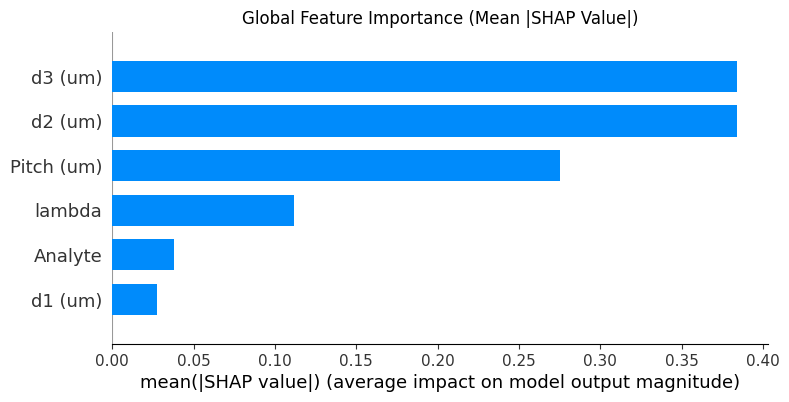
\includegraphics[width=0.45\textwidth]{feature_importance_bar.png}}
\caption{Global feature importance ranking derived from SHAP values.}
\label{fig:shap}
\end{figure}

\section{Engineering Validation}
To verify the physical consistency of the SVR model beyond simple error metrics, we performed an engineering validation by predicting the complete spectral loss response for varying analytes. As shown in Fig. \ref{fig:sensitivity}, the model accurately captures the resonance peak shifts as the analyte refractive index ($n_a$) increases from 1.33 to 1.36.

The predicted average spectral sensitivity is 27.63 nm/RIU (Refractive Index Unit). While this value is relatively low compared to ultra-sensitive optimized designs in literature, it is highly consistent with the specific geometric parameters of the base design used for this validation fold. More importantly, the graph proves that the model correctly understands the phase-matching condition between the fiber mode and the surface plasmon polariton (SPP). As $n_a$ increases, the resonance wavelength ($\lambda_{res}$) shifts toward longer wavelengths (redshift), which is a characteristic behavior of PCF-SPR sensors.

The model's ability to maintain these linear shifts across the entire spectral range, despite the highly non-linear nature of the individual loss curves, demonstrates that it has not merely "memorized" the dataset but has instead captured the fundamental physical relationships governing the sensor's operation. This confirms that the proposed SVR is a reliable surrogate model for rapid sensor optimization.

\begin{figure}[htbp]
\centerline{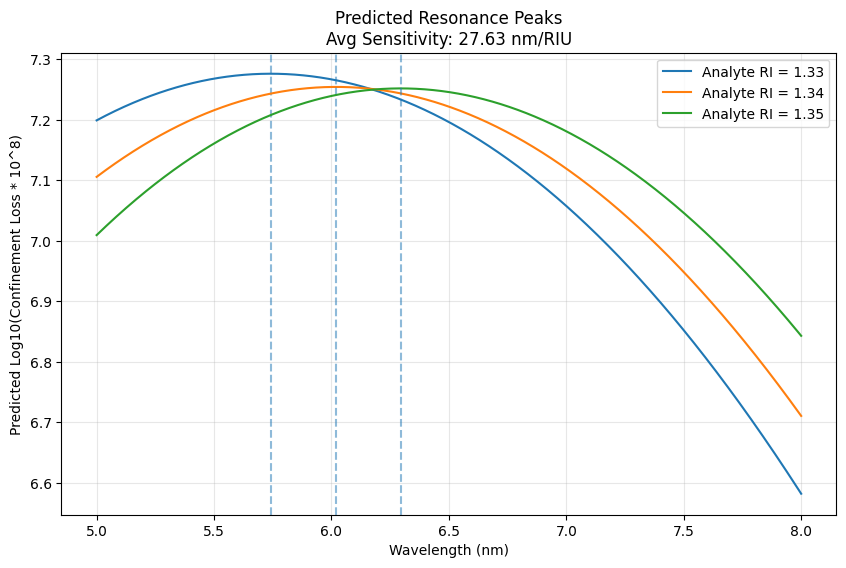
\includegraphics[width=0.45\textwidth]{spectral_sensitivity_curves.png}}
\caption{Predicted resonance peak shifts for varying analytes, demonstrating the model's ability to capture the physical phase-matching behavior.}
\label{fig:sensitivity}
\end{figure}

\section{Conclusion}
In this work, we demonstrate that Bayesian-optimized Support Vector Regression (SVR) and Gaussian Process Regression (GPR) models significantly outperform GAN-augmented neural networks for Photonic Crystal Fiber-Surface Plasmon Resonance (PCF-SPR) sensor modeling. We empirically identify an "Augmentation Paradox," where the non-physical numerical noise inherent to GAN-generated synthetic samples active harms the predictive performance of kernel-based models, suggesting that small-data regimes in photonics are better suited for boundary-focused algorithms than generative deep learning. 

Furthermore, by integrating SHAP analysis and Monte Carlo simulations, we move beyond "black box" modeling to provide actionable engineering insights. Our robustness analysis identifies the sensor pitch ($\Lambda$) as the primary driver of manufacturing instability, accounting for over 90\% of resonance jitter (1.23 nm at 3\% tolerance). This research underscores that high-accuracy predictive modeling, when paired with explainable AI and robustness analysis, can effectively guide the design of next-generation PCF-SPR sensors while minimizing computational costs and ensuring manufacturing reliability.

\begin{thebibliography}{00}
\bibitem{b2} S. Chugh, A. Gulistan, S. Ghosh, and B. M. A. Rahman, ``Machine learning approach for computing optical properties of a photonic crystal fiber,'' \textit{Optics Express}, vol. 27, no. 25, pp. 36414--36425, 2019.
\bibitem{b1} A. Zelaci, A. Yasli, C. Kalyoncu, and H. Ademgil, ``Generative Adversarial Neural Networks Model of Photonic Crystal Fiber Based Surface Plasmon Resonance Sensor,'' \textit{J. Lightwave Technol.}, vol. 39, no. 5, pp. 1515--1522, 2021.
\bibitem{b3} M. R. Khatun and M. S. Islam, ``Design optimization of high-sensitivity PCF-SPR biosensor using machine learning and explainable AI,'' \textit{PLOS ONE}, vol. 20, no. 9, p. e0330944, 2025.
\bibitem{b4} Y. Kizilkaya and C. Kalyoncu, ``Determination of confinement loss characteristics of bent photonic crystal fibers using k-nearest neighbor regression,'' \textit{Laser Phys.}, vol. 32, no. 4, p. 045203, 2022.
\bibitem{b5} A. A. Rifat et al., ``Photonic crystal fiber based plasmonic sensors,'' \textit{Sensors and Actuators B: Chemical}, vol. 243, pp. 311--325, 2017.
\bibitem{b6} P. B. Johnson and R. W. Christy, ``Optical Constants of the Noble Metals,'' \textit{Phys. Rev. B}, vol. 6, no. 12, pp. 4370--4379, 1972.
\bibitem{b7} C. E. Rasmussen and C. K. I. Williams, \textit{Gaussian Processes for Machine Learning}, MIT Press, 2006.
\end{thebibliography}

\end{document}
